\documentclass{ximera}
%verbeterd 22/10/26
\title{Vraagstukken wetten van Newton: meerdere massa's}
\author{Daan Lipkens}

% hulpcommando's voor krachtendiagrammen in de oplossingen (lichamen als puntmassa)
\newcommand{\blokje}[4][left]{\fill (#2,#3) circle (0.05); \node[#1, inner sep=3pt] at (#2,#3) {#4};}
\newcommand{\kr}[7][kracht]{\draw[#1] (#2,#3) -- ++(#4,#5) node[#6] {#7};}

\begin{document}
\begin{abstract}
    Moeilijkere oefeningen op de wetten van Newton met meerdere massa's, van makkelijk naar moeilijk.
\end{abstract}
\maketitle
\section{Oefeningen met meerdere massa's}

Neem in alle oefeningen $g = 9{,}81 \, \mathrm{m/s^2}$. Touwen en katrollen hebben geen massa en de katrollen draaien zonder wrijving, tenzij anders vermeld.

%———————————————————————————————————————
% OEFENING 1: DRIE BLOKKEN TEGEN ELKAAR (contactkrachten + wrijving)
\begin{exercise}
    Drie blokken liggen tegen elkaar op een horizontale tafel. Blok $A$ ($m_{A}= 4{,}0 \, \mathrm{kg}$) wordt horizontaal naar rechts geduwd met een kracht $F = 45 \, \mathrm{N}$. Blok $B$ heeft een massa $m_{B}= 6{,}0 \, \mathrm{kg}$ en blok $C$ een massa $m_{C}= 2{,}0 \, \mathrm{kg}$. De dynamische wrijvingscoëfficiënt tussen de tafel en blok $A$, $B$ en $C$ is respectievelijk $0{,}10$, $0{,}30$ en $0{,}20$.

    \begin{center}
        \begin{tikzpicture}
            \useasboundingbox (-1.5, -0.5) rectangle (6.5, 1.5);
            \draw[thick] (-0.5,0) -- (5.5,0);
            \foreach \x in {-0.3,0,...,5.4} \draw (\x,0) -- ++(-0.15,-0.2);
            \draw[fill=gray!20] (0.8,0) rectangle (2.2,1.0) node[midway] {$m_{A}$};
            \draw[fill=gray!20] (2.2,0) rectangle (4.2,1.0) node[midway] {$m_{B}$};
            \draw[fill=gray!20] (4.2,0) rectangle (5.0,1.0) node[midway] {$m_{C}$};
            \draw[kracht] (-0.8,0.5) -- (0.8,0.5) node[midway, above] {$\vec{F}$};
        \end{tikzpicture}
    \end{center}

    \begin{question}
        Bereken de grootte van de versnelling van de blokken.

        \[ a = \answer[tolerance=0.05,onlineshowanswerbutton]{1.6} \, \mathrm{m/s^2} \]

        \begin{hint}
            Beschouw de drie blokken als één geheel. Welke krachten tussen de blokken onderling moet je dan niet meenemen? Let op: elk blok heeft zijn eigen wrijvingskracht.
        \end{hint}

        \begin{solution}\nl
            \underline{Gegevens:}
            \begin{align*}
                & m_{A} = 4{,}0 \, \mathrm{kg} & & m_{B} = 6{,}0 \, \mathrm{kg} \\
                & m_{C} = 2{,}0 \, \mathrm{kg} & & F = 45 \, \mathrm{N} \\
                & \mu_{A} = 0{,}10 & & \mu_{B} = 0{,}30 \\
                & \mu_{C} = 0{,}20 & & g = 9{,}81 \, \mathrm{m/s^2}
            \end{align*}

            \underline{Gevraagd:} $a$ \\

            \underline{Oplossing:}\\
            Alle blokken voeren dezelfde beweging uit, dus we beschouwen ze als één systeem. De krachten tussen de blokken zijn dan inwendige krachten en vallen weg. Verticaal is er evenwicht, dus $F_{N} = m \cdot g$ voor elk blok en de wrijvingskracht is $F_{w,d} = \mu \cdot m \cdot g$:
            \begin{align*}
                F_{w,d,A} &= 0{,}10 \cdot 4{,}0 \, \mathrm{kg} \cdot 9{,}81 \, \mathrm{m/s^2} = 3{,}924 \, \mathrm{N} \\
                F_{w,d,B} &= 0{,}30 \cdot 6{,}0 \, \mathrm{kg} \cdot 9{,}81 \, \mathrm{m/s^2} = 17{,}658 \, \mathrm{N} \\
                F_{w,d,C} &= 0{,}20 \cdot 2{,}0 \, \mathrm{kg} \cdot 9{,}81 \, \mathrm{m/s^2} = 3{,}924 \, \mathrm{N}
            \end{align*}
            De tweede wet van Newton, geprojecteerd op de horizontale as (positief naar rechts):
            \begin{align*}
                F - F_{w,d,A} - F_{w,d,B} - F_{w,d,C} &= (m_{A}+m_{B}+m_{C}) \cdot a \\
                a &= \frac{45 \, \mathrm{N} - 3{,}924 \, \mathrm{N} - 17{,}658 \, \mathrm{N} - 3{,}924 \, \mathrm{N}}{12{,}0 \, \mathrm{kg}} \\
                &= 1{,}6245 \, \mathrm{m/s^2} \simeq 1{,}6 \, \mathrm{m/s^2}
            \end{align*}
        \end{solution}
    \end{question}

    \begin{question}
        Bereken de grootte van de kracht die blok $A$ uitoefent op blok $B$ en van de kracht die blok $B$ uitoefent op blok $C$.

        \[ F_{AB} = \answer[tolerance=0.03,onlineshowanswerbutton]{34.6} \, \mathrm{N} \qquad F_{BC} = \answer[tolerance=0.03,onlineshowanswerbutton]{7.2} \, \mathrm{N} \]

        \begin{hint}
            Bekijk blok $C$ afzonderlijk: welke horizontale krachten werken er op en welke versnelling heeft het? Voor $F_{AB}$ kan je blok $A$ afzonderlijk bekijken. Wat zegt de derde wet over de kracht van $B$ op $A$?
        \end{hint}

        \begin{solution}\nl
            \underline{Gevraagd:} $F_{AB}$ en $F_{BC}$ \\

            \underline{Oplossing:}\\
            \begin{center}
            \begin{tikzpicture}
            \blokje[below right]{0}{0}{$m_{A}$}
            \kr[kracht]{0}{0}{0}{0.9}{right}{$\vec{\mathbf{F}}_{N}$}
            \kr[kracht]{0}{0}{0}{-0.9}{right}{$\vec{\mathbf{F}}_{z}$}
            \kr[versnelling]{-0.4}{1.6}{0.8}{0}{above}{$\vec{\mathbf{a}}$}
            \blokje[below right]{4.5}{0}{$m_{B}$}
            \kr[kracht]{4.5}{0}{0}{0.9}{right}{$\vec{\mathbf{F}}_{N}$}
            \kr[kracht]{4.5}{0}{0}{-0.9}{right}{$\vec{\mathbf{F}}_{z}$}
            \kr[versnelling]{4.1}{1.6}{0.8}{0}{above}{$\vec{\mathbf{a}}$}
            \blokje[below right]{9}{0}{$m_{C}$}
            \kr[kracht]{9}{0}{0}{0.9}{right}{$\vec{\mathbf{F}}_{N}$}
            \kr[kracht]{9}{0}{0}{-0.9}{right}{$\vec{\mathbf{F}}_{z}$}
            \kr[versnelling]{8.6}{1.6}{0.8}{0}{above}{$\vec{\mathbf{a}}$}
            \kr[kracht]{0}{0.1}{1.8}{0}{pos=0.6,above}{$\vec{\mathbf{F}}$}
            \kr[kracht]{0}{0.1}{-1.38}{0}{pos=0.5,above}{$\vec{\mathbf{F}}_{BA}$}
            \kr[kracht]{0}{-0.1}{-0.55}{0}{pos=0.5,below}{$\vec{\mathbf{F}}_{w,d,A}$}
            \kr[kracht]{4.5}{0.1}{1.38}{0}{pos=0.5,above}{$\vec{\mathbf{F}}_{AB}$}
            \kr[kracht]{4.5}{0.1}{-0.55}{0}{pos=0.5,above}{$\vec{\mathbf{F}}_{CB}$}
            \kr[kracht]{4.5}{-0.1}{-0.9}{0}{pos=0.5,below}{$\vec{\mathbf{F}}_{w,d,B}$}
            \kr[kracht]{9}{0.1}{0.6}{0}{right}{$\vec{\mathbf{F}}_{BC}$}
            \kr[kracht]{9}{-0.1}{-0.55}{0}{pos=0.5,below}{$\vec{\mathbf{F}}_{w,d,C}$}
            \end{tikzpicture}
            \end{center}

            Blok $C$ wordt enkel naar rechts geduwd door blok $B$ ($F_{BC}$) en naar links afgeremd door de wrijving $F_{w,d,C}$:
            \begin{align*}
                F_{BC} - F_{w,d,C} &= m_{C} \cdot a \\
                F_{BC} &= 2{,}0 \, \mathrm{kg} \cdot 1{,}6245 \, \mathrm{m/s^2} + 3{,}924 \, \mathrm{N} \\
                &= 7{,}173 \, \mathrm{N} \simeq 7{,}2 \, \mathrm{N}
            \end{align*}
            Op blok $A$ werken $F$ (naar rechts), de wrijving $F_{w,d,A}$ en de kracht $F_{BA}$ van blok $B$ op $A$ (naar links). Volgens de derde wet is $F_{BA} = F_{AB}$:
            \begin{align*}
                F - F_{w,d,A} - F_{AB} &= m_{A} \cdot a \\
                F_{AB} &= 45 \, \mathrm{N} - 3{,}924 \, \mathrm{N} - 4{,}0 \, \mathrm{kg} \cdot 1{,}6245 \, \mathrm{m/s^2} \\
                &= 34{,}578 \, \mathrm{N} \simeq 34{,}6 \, \mathrm{N}
            \end{align*}
            Controle met blok $B$: $F_{AB} - F_{w,d,B} - F_{BC} = 34{,}578 \, \mathrm{N} - 17{,}658 \, \mathrm{N} - 7{,}173 \, \mathrm{N} = 9{,}747 \, \mathrm{N} = m_{B} \cdot a$. 
        \end{solution}
    \end{question}

    \begin{question}
        De kracht $F = 45 \, \mathrm{N}$ wordt nu horizontaal naar links uitgeoefend op blok $C$ (de volgorde $A$, $B$, $C$ van links naar rechts blijft behouden). Bereken de grootte van de kracht tussen blok $B$ en blok $C$.

        \[ F_{CB} = \answer[tolerance=0.02,onlineshowanswerbutton]{37.8} \, \mathrm{N} \]

        \begin{hint}
            De versnelling van het geheel verandert niet. Welke blokken worden nu door blok $C$ meegeduwd? Bekijk die blokken samen als één deelsysteem.
        \end{hint}

        \begin{solution}\nl
            \underline{Gevraagd:} $F_{CB}$ \\

            \underline{Oplossing:}\\
            De totale massa en de totale wrijving zijn ongewijzigd, dus de versnelling is nog steeds $1{,}6245 \, \mathrm{m/s^2}$ (nu naar links). Blok $C$ duwt blok $B$, en blok $B$ duwt blok $A$. We bekijken blok $B$ en $A$ samen als deelsysteem. De enige uitwendige krachten in de bewegingsrichting zijn $F_{CB}$ en de wrijvingen $F_{w,d,A}$ en $F_{w,d,B}$:
            \begin{align*}
                F_{CB} - F_{w,d,A} - F_{w,d,B} &= (m_{A}+m_{B}) \cdot a \\
                F_{CB} &= 10{,}0 \, \mathrm{kg} \cdot 1{,}6245 \, \mathrm{m/s^2} + 3{,}924 \, \mathrm{N} + 17{,}658 \, \mathrm{N} \\
                &= 37{,}827 \, \mathrm{N} \simeq 37{,}8 \, \mathrm{N}
            \end{align*}
            De contactkracht tussen $B$ en $C$ hangt dus af van langs welke kant je duwt.
        \end{solution}
    \end{question}
\end{exercise}
%———————————————————————————————————————

%———————————————————————————————————————
% OEFENING 2: ATWOOD MET DRIE MASSA'S
\begin{exercise}
    Over een vaste katrol loopt een touw (touw 1). Aan het ene uiteinde hangt een blok met massa $m_{1}= 1{,}2 \, \mathrm{kg}$. Aan het andere uiteinde hangt een blok met massa $m_{2}= 0{,}40 \, \mathrm{kg}$. Onder dat blok hangt via een tweede touw (touw 2) een blok met massa $m_{3}= 200 \, \mathrm{g}$. Het systeem wordt losgelaten.

    \begin{center}
        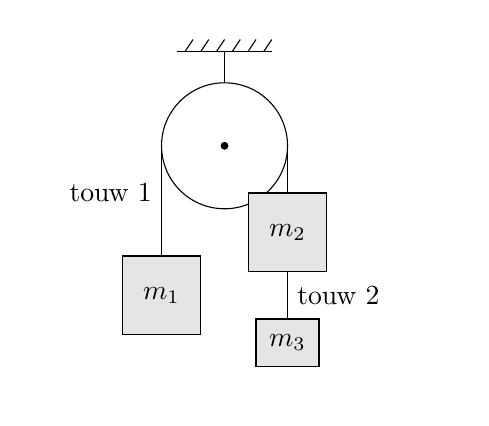
\begin{tikzpicture}
            \useasboundingbox (-2.5, -0.2) rectangle (3, 4.5);
            \draw (-0.6,4.2) -- (0.6,4.2);
            \foreach \x in {-0.5,-0.3,...,0.5} \draw (\x,4.2) -- ++(0.1,0.15);
            \draw (0,4.2) -- (0,3);
            \draw[fill=white] (0,3) circle (0.8);
            \fill (0,3) circle (0.05);
            \draw (-0.8,3) -- (-0.8,1.6);
            \draw (0.8,3) -- (0.8,2.4);
            \draw[fill=gray!20] (-1.3,0.6) rectangle (-0.3,1.6) node[midway] {$m_{1}$};
            \draw[fill=gray!20] (0.3,1.4) rectangle (1.3,2.4) node[midway] {$m_{2}$};
            \draw (0.8,1.4) -- (0.8,0.8);
            \draw[fill=gray!20] (0.4,0.2) rectangle (1.2,0.8) node[midway] {$m_{3}$};
            \node[left] at (-0.8,2.4) {touw 1};
            \node[right] at (0.8,1.1) {touw 2};
        \end{tikzpicture}
    \end{center}

    \begin{question}
        Bereken de grootte van de versnelling van de blokken.

        \[ a = \answer[tolerance=0.02,onlineshowanswerbutton]{3.27} \, \mathrm{m/s^2} \]

        \begin{hint}
            Alle touwen blijven gespannen, dus alle blokken hebben een versnelling met dezelfde grootte. Je kan de drie blokken samen als één systeem bekijken. Welke krachten vallen dan weg?
        \end{hint}

        \begin{solution}\nl
            \underline{Gegevens:}
            \begin{align*}
                & m_{1} = 1{,}2 \, \mathrm{kg} & & m_{2} = 0{,}40 \, \mathrm{kg} \\
                & m_{3} = 200 \, \mathrm{g} = 0{,}20 \, \mathrm{kg} & & g = 9{,}81 \, \mathrm{m/s^2}
            \end{align*}

            \underline{Gevraagd:} $a$ \\

            \underline{Oplossing:}\\
            \begin{center}
            \begin{tikzpicture}
            \blokje[left,xshift=-0.15cm]{0}{0}{$m_{1}$}
            \blokje[left,xshift=-0.15cm]{3}{0}{$m_{2}$}
            \blokje[left,xshift=-0.15cm]{6}{0}{$m_{3}$}
            \kr[kracht]{0}{0}{0}{1.1}{right}{$\vec{\mathbf{F}}_{t,1}$}
            \kr[kracht]{0}{0}{0}{-1.65}{right}{$\vec{\mathbf{F}}_{z,1}$}
            \kr[kracht]{2.85}{0}{0}{1.1}{left}{$\vec{\mathbf{F}}_{t,1}$}
            \kr[kracht]{2.85}{0}{0}{-0.55}{left}{$\vec{\mathbf{F}}_{z,2}$}
            \kr[kracht]{3.15}{0}{0}{-0.37}{right}{$\vec{\mathbf{F}}_{t,2}$}
            \kr[kracht]{6}{0}{0}{0.37}{right}{$\vec{\mathbf{F}}_{t,2}$}
            \kr[kracht]{6}{0}{0}{-0.27}{right}{$\vec{\mathbf{F}}_{z,3}$}
            \kr[versnelling]{0.9}{0.2}{0}{-0.8}{right}{$\vec{\mathbf{a}}$}
            \kr[versnelling]{3.9}{-0.2}{0}{0.8}{right}{$\vec{\mathbf{a}}$}
            \kr[versnelling]{6.9}{-0.2}{0}{0.8}{right}{$\vec{\mathbf{a}}$}
            \end{tikzpicture}
            \end{center}

            Blok 1 zakt, blok 2 en 3 stijgen. We nemen de bewegingsrichting als positief. Voor de drie blokken afzonderlijk:
            \begin{align*}
                m_{1} \cdot g - F_{t,1} &= m_{1} \cdot a \\
                F_{t,1} - m_{2} \cdot g - F_{t,2} &= m_{2} \cdot a \\
                F_{t,2} - m_{3} \cdot g &= m_{3} \cdot a
            \end{align*}
            Optellen van de drie vergelijkingen laat de spankrachten wegvallen:
            \begin{align*}
                (m_{1} - m_{2} - m_{3}) \cdot g &= (m_{1}+m_{2}+m_{3}) \cdot a \\
                a &= \frac{(1{,}2 \, \mathrm{kg} - 0{,}40 \, \mathrm{kg} - 0{,}20 \, \mathrm{kg}) \cdot 9{,}81 \, \mathrm{m/s^2}}{1{,}2 \, \mathrm{kg} + 0{,}40 \, \mathrm{kg} + 0{,}20 \, \mathrm{kg}} \\
                &= 3{,}27 \, \mathrm{m/s^2}
            \end{align*}
        \end{solution}
    \end{question}

    \begin{question}
        Bereken de spankracht in touw 1 en in touw 2.

        \[ F_{t,1} = \answer[tolerance=0.02,onlineshowanswerbutton]{7.85} \, \mathrm{N} \qquad F_{t,2} = \answer[tolerance=0.02,onlineshowanswerbutton]{2.62} \, \mathrm{N} \]

        \begin{hint}
            Kies telkens het blok waarvoor je de minste krachten moet bijhouden. Welk blok is dat voor $F_{t,1}$ en welk voor $F_{t,2}$?
        \end{hint}

        \begin{solution}\nl
            \underline{Gevraagd:} $F_{t,1}$ en $F_{t,2}$ \\

            \underline{Oplossing:}\\
            Uit de vergelijking van blok 1 en van blok 3:
            \begin{align*}
                F_{t,1} &= m_{1} \cdot (g - a) = 1{,}2 \, \mathrm{kg} \cdot (9{,}81 \, \mathrm{m/s^2} - 3{,}27 \, \mathrm{m/s^2}) = 7{,}848 \, \mathrm{N} \simeq 7{,}85 \, \mathrm{N} \\
                F_{t,2} &= m_{3} \cdot (g + a) = 0{,}20 \, \mathrm{kg} \cdot (9{,}81 \, \mathrm{m/s^2} + 3{,}27 \, \mathrm{m/s^2}) = 2{,}616 \, \mathrm{N} \simeq 2{,}62 \, \mathrm{N}
            \end{align*}
            Controle met blok 2: $F_{t,1} - m_{2} \cdot g - F_{t,2} = 7{,}848 \, \mathrm{N} - 3{,}924 \, \mathrm{N} - 2{,}616 \, \mathrm{N} = 1{,}308 \, \mathrm{N} = m_{2} \cdot a$. 
        \end{solution}
    \end{question}

    \begin{question}
        Op een bepaald moment breekt touw 2. Bereken de grootte van de versnelling van blok 1 en de spankracht in touw 1 vlak daarna.

        \[ a' = \answer[tolerance=0.02,onlineshowanswerbutton]{4.9} \, \mathrm{m/s^2} \qquad F_{t,1}' = \answer[tolerance=0.02,onlineshowanswerbutton]{5.9} \, \mathrm{N} \]

        \begin{hint}
            Blok 3 hoort er niet meer bij. Welke blokken blijven er over in het systeem dat via touw 1 verbonden is?
        \end{hint}

        \begin{solution}\nl
            \underline{Gevraagd:} $a'$ en $F_{t,1}'$ \\

            \underline{Oplossing:}\\
            Enkel blok 1 en blok 2 blijven verbonden:
            \begin{align*}
                a' &= \frac{(m_{1} - m_{2}) \cdot g}{m_{1}+m_{2}} = \frac{(1{,}2 \, \mathrm{kg} - 0{,}40 \, \mathrm{kg}) \cdot 9{,}81 \, \mathrm{m/s^2}}{1{,}2 \, \mathrm{kg} + 0{,}40 \, \mathrm{kg}} = 4{,}905 \, \mathrm{m/s^2} \simeq 4{,}9 \, \mathrm{m/s^2} \\
                F_{t,1}' &= m_{1} \cdot (g - a') = 1{,}2 \, \mathrm{kg} \cdot (9{,}81 \, \mathrm{m/s^2} - 4{,}905 \, \mathrm{m/s^2}) = 5{,}886 \, \mathrm{N} \simeq 5{,}9 \, \mathrm{N}
            \end{align*}
            De spankracht in touw 1 is kleiner geworden: blok 2 moet nu minder massa meetrekken.
        \end{solution}
    \end{question}
\end{exercise}
%———————————————————————————————————————

%———————————————————————————————————————
% OEFENING 3: HELLING + HANGEND BLOK, RUST OF BEWEGING
\begin{exercise}
    Een blok met massa $m_{1}= 5{,}0 \, \mathrm{kg}$ ligt op een helling van $30^\circ$. Het blok is via een touw dat evenwijdig met de helling loopt en over een katrol bovenaan de helling gaat, verbonden met een hangend blok met massa $m_{2}$. De statische wrijvingscoëfficiënt tussen blok 1 en de helling is $0{,}40$ en de dynamische wrijvingscoëfficiënt is $0{,}30$. Het systeem wordt losgelaten vanuit rust.

    \begin{center}
        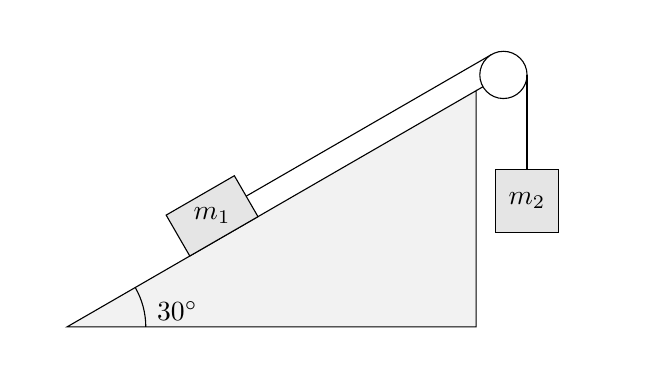
\begin{tikzpicture}
            \useasboundingbox (-0.5, -0.3) rectangle (7, 3.8);
            \draw[fill=gray!10] (0,0) -- (5.196,0) -- (5.196,3) -- cycle;
            \draw (1,0) arc (0:30:1);
            \node at (1.4,0.2) {$30^\circ$};
            \begin{scope}[rotate=30]
                \draw[fill=gray!20] (1.8,0) rectangle (2.8,0.6) node[midway] {$m_{1}$};
                \draw (2.8,0.3) -- (6.4,0.3);
            \end{scope}
            \draw (5.196,3) -- (5.542,3.2);
            \draw[fill=white] (5.542,3.2) circle (0.3);
            \draw (5.842,3.2) -- (5.842,2.0);
            \draw[fill=gray!20] (5.442,1.2) rectangle (6.242,2.0) node[midway] {$m_{2}$};
        \end{tikzpicture}
    \end{center}

    \begin{question}
        Eerst is $m_{2} = 1{,}0 \, \mathrm{kg}$. Wat gebeurt er met het systeem?

        \wordChoice{
            \choice[correct]{Het blijft in rust.}
            \choice{Blok 1 glijdt omlaag langs de helling.}
            \choice{Blok 1 glijdt omhoog langs de helling.}
        }

        \begin{hint}
            Bepaal welke kracht er nodig is om blok 1 in rust te houden (naast de spankracht) en vergelijk die met de grootste statische wrijvingskracht die de helling kan leveren.
        \end{hint}

        \begin{solution}\nl
            \underline{Gegevens:}
            \begin{align*}
                & m_{1} = 5{,}0 \, \mathrm{kg} & & \alpha = 30^\circ \\
                & \mu_{s} = 0{,}40 & & \mu_{d} = 0{,}30 \\
                & g = 9{,}81 \, \mathrm{m/s^2} & &
            \end{align*}

            \underline{Gevraagd:} beweegt het systeem? \\

            \underline{Oplossing:}\\
            \begin{center}
            \begin{tikzpicture}[scale=1.7]
            \begin{scope}[rotate=30]
            \draw[thick] (-3,-0.15) -- (3,-0.15);
            \foreach \x in {-2.8,-2.5,...,2.9} \draw (\x,-0.15) -- ++(-0.12,-0.2);
            \node[left, inner sep=4pt] at (0,0) {$m_{1}$};
            \fill (0,0) circle (0.04);
            \draw[kracht] (0,0) -- (0,1.7) node[above left] {$\vec{\mathbf{F}}_{N}$};
            \draw[kracht] (0,0.12) -- (0.39,0.12) node[right] {$\vec{\mathbf{F}}_{t}$};
            \draw[kracht] (0,-0.12) -- (0.59,-0.12) node[right] {$\vec{\mathbf{F}}_{w,s}$};
            \draw[kracht] (0,0) -- (-0.98,-1.70) node[below] {$\vec{\mathbf{F}}_{z,1}$};
            \draw[krachtcomponent] (0,0) -- (-0.98,0) node[above left] {$\vec{\mathbf{F}}_{z,1,x}$};
            \draw[krachtcomponent] (0,0) -- (0,-1.70) node[below right] {$\vec{\mathbf{F}}_{z,1,y}$};
            \draw[dashed,gray] (-0.98,0) -- (-0.98,-1.70) -- (0,-1.70);
            \draw (0,-0.6) arc[start angle=-90,end angle=-120,radius=0.6];
            \node at (-0.2,-0.95) {\scriptsize $30^\circ$};
            \draw (-0.5,0) arc[start angle=180,end angle=240,radius=0.5];
            \node at (-0.85,-0.32) {\scriptsize $60^\circ$};
            \end{scope}
            \end{tikzpicture}
            \end{center}

            We kiezen een $x$-as evenwijdig met de helling en een $y$-as loodrecht erop. De hoek tussen $\vec{\mathbf{F}}_{z,1}$ en de $x$-as is $60^\circ$ en de hoek met de $y$-as is $30^\circ$. De componenten van de zwaartekracht op blok 1 zijn:
            \begin{align*}
                F_{z,1,x} &= m_{1} \cdot g \cdot \cos(60^\circ) = 5{,}0 \, \mathrm{kg} \cdot 9{,}81 \, \mathrm{m/s^2} \cdot \cos(60^\circ) = 24{,}525 \, \mathrm{N} \\
                F_{z,1,y} &= m_{1} \cdot g \cdot \cos(30^\circ) = 42{,}479 \, \mathrm{N}
            \end{align*}
            Loodrecht op de helling is er evenwicht, dus $F_{N} = 42{,}479 \, \mathrm{N}$. De grootst mogelijke statische wrijving is:
            \[
                F_{w,s,\max} = \mu_{s} \cdot F_{N} = 0{,}40 \cdot 42{,}479 \, \mathrm{N} = 16{,}99 \, \mathrm{N}
            \]
            Zonder wrijving zou blok 1 langs de helling omlaag getrokken worden met een nettokracht van
            \[
                F_{z,1,x} - m_{2} \cdot g = 24{,}525 \, \mathrm{N} - 1{,}0 \, \mathrm{kg} \cdot 9{,}81 \, \mathrm{m/s^2} = 14{,}715 \, \mathrm{N}
            \]
            Omdat $14{,}715 \, \mathrm{N} < 16{,}99 \, \mathrm{N}$ kan de statische wrijving dit tegenhouden: het systeem blijft in rust.
        \end{solution}
    \end{question}

    \begin{question}
        Bereken de grootte van de statische wrijvingskracht op blok 1 als $m_{2} = 1{,}0 \, \mathrm{kg}$.

        \[ F_{w,s} = \answer[tolerance=0.02,onlineshowanswerbutton]{14.7} \, \mathrm{N} \]

        \begin{hint}
            Het systeem is in rust. Wat is dan de spankracht in het touw, en wat betekent dat voor het evenwicht van blok 1 langs de helling?
        \end{hint}

        \begin{solution}\nl
            \underline{Gevraagd:} $F_{w,s}$ \\

            \underline{Oplossing:}\\
            Blok 2 is in rust, dus $F_{t} = m_{2} \cdot g = 9{,}81 \, \mathrm{N}$. Langs de helling is blok 1 in evenwicht. De zwaartekrachtcomponent wijst omlaag, de spankracht en de statische wrijving wijzen omhoog:
            \begin{align*}
                F_{z,1,x} - F_{t} - F_{w,s} &= 0 \\
                F_{w,s} &= 24{,}525 \, \mathrm{N} - 9{,}81 \, \mathrm{N} = 14{,}715 \, \mathrm{N} \simeq 14{,}7 \, \mathrm{N}
            \end{align*}
            De statische wrijving is hier dus kleiner dan het maximum ($16{,}99 \, \mathrm{N}$): ze past zich aan wat nodig is.
        \end{solution}
    \end{question}

    \begin{question}
        Nu wordt blok 2 vervangen door een blok van $400 \, \mathrm{g}$. Bereken de grootte van de versnelling van de blokken en de spankracht in het touw.

        \[ a = \answer[tolerance=0.03,onlineshowanswerbutton]{1.46} \, \mathrm{m/s^2} \qquad F_{t} = \answer[tolerance=0.03,onlineshowanswerbutton]{4.5} \, \mathrm{N} \]

        \begin{hint}
            Controleer eerst of het systeem nog in rust kan blijven. Maak daarna voor elk blok een tekening met alle krachten en kies voor elk blok een positieve zin die overeenkomt met zijn bewegingsrichting.
        \end{hint}

        \begin{solution}\nl
            \underline{Gegevens:} $m_{2} = 400 \, \mathrm{g} = 0{,}40 \, \mathrm{kg}$, de andere gegevens zijn ongewijzigd. \\

            \underline{Gevraagd:} $a$ en $F_{t}$ \\

            \underline{Oplossing:}\\
            Eerst controleren we of het systeem beweegt: de nettokracht langs de helling is nu
            \[
                24{,}525 \, \mathrm{N} - 0{,}40 \, \mathrm{kg} \cdot 9{,}81 \, \mathrm{m/s^2} = 20{,}601 \, \mathrm{N} > F_{w,s,\max} = 16{,}99 \, \mathrm{N}
            \]
            Blok 1 glijdt dus omlaag en blok 2 stijgt. De wrijving is nu dynamisch en wijst omhoog langs de helling, tegengesteld aan de beweging van blok 1:
            \[
                F_{w,d} = \mu_{d} \cdot F_{N} = 0{,}30 \cdot 42{,}479 \, \mathrm{N} = 12{,}744 \, \mathrm{N}
            \]

            \begin{center}
\begin{tikzpicture}[scale=1.7]
\begin{scope}[rotate=30]
\draw[thick] (-3,-0.15) -- (3,-0.15);
\foreach \x in {-2.8,-2.5,...,2.9} \draw (\x,-0.15) -- ++(-0.12,-0.2);
\node[left, inner sep=4pt] at (0,0) {$m_{1}$};
\fill (0,0) circle (0.04);
\draw[kracht] (0,0) -- (0,1.7) node[above left] {$\vec{\mathbf{F}}_{N}$};
\draw[kracht] (0,0.12) -- (0.18,0.12) node[right] {$\vec{\mathbf{F}}_{t}$};
\draw[kracht] (0,-0.12) -- (0.51,-0.12) node[right] {$\vec{\mathbf{F}}_{w,d}$};
\draw[kracht] (0,0) -- (-0.98,-1.70) node[below] {$\vec{\mathbf{F}}_{z,1}$};
\draw[krachtcomponent] (0,0) -- (-0.98,0) node[above left] {$\vec{\mathbf{F}}_{z,1,x}$};
\draw[krachtcomponent] (0,0) -- (0,-1.70) node[below right] {$\vec{\mathbf{F}}_{z,1,y}$};
\draw[dashed,gray] (-0.98,0) -- (-0.98,-1.70) -- (0,-1.70);
\draw (0,-0.6) arc[start angle=-90,end angle=-120,radius=0.6];
\node at (-0.2,-0.95) {\scriptsize $30^\circ$};
\draw (-0.5,0) arc[start angle=180,end angle=240,radius=0.5];
\node at (-0.85,-0.32) {\scriptsize $60^\circ$};
\draw[versnelling] (0.9,0.6) -- (0.2,0.6) node[above] {$\vec{\mathbf{a}}$};
\end{scope}
\end{tikzpicture}
\end{center}

            Voor blok 1 projecteren we op de $x$-as (positief omlaag langs de helling) en voor blok 2 op een verticale as (positief omhoog):
            \begin{align*}
                F_{z,1,x} - F_{t} - F_{w,d} &= m_{1} \cdot a \\
                F_{t} - m_{2} \cdot g &= m_{2} \cdot a
            \end{align*}
            Optellen en oplossen naar $a$:
            \begin{align*}
                a &= \frac{F_{z,1,x} - m_{2} \cdot g - F_{w,d}}{m_{1}+m_{2}} \\
                &= \frac{24{,}525 \, \mathrm{N} - 3{,}924 \, \mathrm{N} - 12{,}744 \, \mathrm{N}}{5{,}0 \, \mathrm{kg} + 0{,}40 \, \mathrm{kg}} = 1{,}455 \, \mathrm{m/s^2} \simeq 1{,}46 \, \mathrm{m/s^2}
            \end{align*}
            Daarna is de spankracht:
            \[
                F_{t} = m_{2} \cdot (g + a) = 0{,}40 \, \mathrm{kg} \cdot (9{,}81 \, \mathrm{m/s^2} + 1{,}455 \, \mathrm{m/s^2}) = 4{,}506 \, \mathrm{N} \simeq 4{,}5 \, \mathrm{N}
            \]
        \end{solution}
    \end{question}
\end{exercise}
%———————————————————————————————————————

%———————————————————————————————————————
% OEFENING 4: VEER TUSSEN TWEE BLOKKEN, TOUW DOORKNIPPEN, LIFT
\begin{exercise}
    Twee blokken hangen onder elkaar aan een touw. Het bovenste blok heeft een massa $m_{1}= 2{,}0 \, \mathrm{kg}$ en het onderste blok een massa $m_{2}= 3{,}0 \, \mathrm{kg}$. De twee blokken zijn met elkaar verbonden door een veer met een veerconstante $k = 2{,}0 \, \mathrm{N/cm}$. De massa van de veer en het touw is verwaarloosbaar.

    \begin{center}
        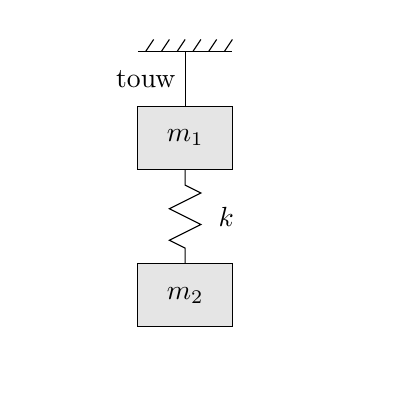
\begin{tikzpicture}
            \useasboundingbox (-2, -0.3) rectangle (2.5, 4.3);
            \draw (-0.6,4.0) -- (0.6,4.0);
            \foreach \x in {-0.5,-0.3,...,0.5} \draw (\x,4.0) -- ++(0.1,0.15);
            \draw (0,4.0) -- (0,3.3);
            \draw[fill=gray!20] (-0.6,2.5) rectangle (0.6,3.3) node[midway] {$m_{1}$};
            \draw (0,2.5) -- (0,2.3) -- (0.2,2.2) -- (-0.2,2.0) -- (0.2,1.8) -- (-0.2,1.6) -- (0,1.5) -- (0,1.3);
            \node[right] at (0.3,1.9) {$k$};
            \draw[fill=gray!20] (-0.6,0.5) rectangle (0.6,1.3) node[midway] {$m_{2}$};
            \node[left] at (0,3.65) {touw};
        \end{tikzpicture}
    \end{center}

    \begin{question}
        Het systeem hangt in rust. Bereken hoeveel de veer is uitgerekt en bereken de spankracht in het touw.

        \[ x = \answer[tolerance=0.02,onlineshowanswerbutton]{14.7} \, \mathrm{cm} \qquad F_{t} = \answer[tolerance=0.02,onlineshowanswerbutton]{49.1} \, \mathrm{N} \]

        \begin{hint}
            Welk blok heeft de veer als enige verbinding met de rest nodig om in rust te blijven? Bekijk de krachten op dat blok. Voor het touw kan je het hele geheel van blokken en veer als één systeem bekijken.
        \end{hint}

        \begin{solution}\nl
            \underline{Gegevens:}
            \begin{align*}
                & m_{1} = 2{,}0 \, \mathrm{kg} & & m_{2} = 3{,}0 \, \mathrm{kg} \\
                & k = 2{,}0 \, \mathrm{N/cm} = 200 \, \mathrm{N/m} & & g = 9{,}81 \, \mathrm{m/s^2}
            \end{align*}

            \underline{Gevraagd:} $x$ en $F_{t}$ \\

            \underline{Oplossing:}\\
            \begin{center}
            \begin{tikzpicture}[scale=1.5]
            \blokje[left,xshift=-0.15cm]{0}{0}{$m_{1}$}
            \blokje[left,xshift=-0.15cm]{3}{0}{$m_{2}$}
            \kr[kracht]{0}{0}{0}{1.47}{right}{$\vec{\mathbf{F}}_{t}$}
            \kr[kracht]{-0.2}{0}{0}{-0.59}{left}{$\vec{\mathbf{F}}_{z,1}$}
            \kr[kracht]{0.2}{0}{0}{-0.88}{right}{$\vec{\mathbf{F}}_{v}$}
            \kr[kracht]{3}{0}{0}{0.88}{right}{$\vec{\mathbf{F}}_{v}$}
            \kr[kracht]{3}{0}{0}{-0.88}{right}{$\vec{\mathbf{F}}_{z,2}$}
            \end{tikzpicture}
            \end{center}

            Blok 2 is in rust: de veerkracht (omhoog) compenseert de zwaartekracht (omlaag):
            \begin{align*}
                k \cdot x - m_{2} \cdot g &= 0 \\
                x &= \frac{3{,}0 \, \mathrm{kg} \cdot 9{,}81 \, \mathrm{m/s^2}}{200 \, \mathrm{N/m}} = 0{,}14715 \, \mathrm{m} \simeq 14{,}7 \, \mathrm{cm}
            \end{align*}
            Voor het touw bekijken we blokken en veer als één systeem. Verticaal werken enkel de spankracht en de zwaartekracht op beide blokken:
            \[
                F_{t} = (m_{1}+m_{2}) \cdot g = 5{,}0 \, \mathrm{kg} \cdot 9{,}81 \, \mathrm{m/s^2} = 49{,}05 \, \mathrm{N} \simeq 49{,}1 \, \mathrm{N}
            \]
        \end{solution}
    \end{question}

    \begin{question}
        Het touw wordt doorgeknipt. Bereken de grootte van de versnelling van beide blokken \emph{net na} het doorknippen.

        \[ a_{1} = \answer[tolerance=0.02,onlineshowanswerbutton]{24.5} \, \mathrm{m/s^2} \qquad a_{2} = \answer[tolerance=0.02,onlineshowanswerbutton]{0} \, \mathrm{m/s^2} \]

        \begin{hint}
            Een veer kan haar lengte niet op één ogenblik veranderen. Wat betekent dat voor de veerkracht op het moment van doorknippen? Teken daarna voor elk blok afzonderlijk alle krachten.
        \end{hint}

        \begin{solution}\nl
            \underline{Gevraagd:} $a_{1}$ en $a_{2}$ \\

            \underline{Oplossing:}\\
            Net na het doorknippen is de veer nog even lang, dus de veerkracht is nog $F_{v} = k \cdot x = m_{2} \cdot g = 29{,}43 \, \mathrm{N}$. 

            Op blok 2 werken de veerkracht (omhoog) en de zwaartekracht (omlaag), die elkaar compenseren: $a_{2} = 0$.

            Op blok 1 werken de zwaartekracht en de veerkracht (de uitgerekte veer trekt blok 1 omlaag), beide omlaag:
            \begin{align*}
                m_{1} \cdot g + F_{v} &= m_{1} \cdot a_{1} \\
                a_{1} &= \frac{2{,}0 \, \mathrm{kg} \cdot 9{,}81 \, \mathrm{m/s^2} + 29{,}43 \, \mathrm{N}}{2{,}0 \, \mathrm{kg}} = 24{,}525 \, \mathrm{m/s^2} \simeq 24{,}5 \, \mathrm{m/s^2}
            \end{align*}
            Blok 1 versnelt dus sterker dan bij vrije val.
        \end{solution}
    \end{question}

    \begin{question}
        Het touw wordt opnieuw aan het plafond van een lift bevestigd. De lift versnelt met $1{,}5 \, \mathrm{m/s^2}$ naar boven en blokken en veer hangen in rust ten opzichte van de lift. Bereken hoeveel de veer nu is uitgerekt.

        \[ x' = \answer[tolerance=0.02,onlineshowanswerbutton]{17.0} \, \mathrm{cm} \]

        \begin{hint}
            Beide blokken versnellen mee met de lift. Welke blok zorgt ervoor dat de veerkracht afwijkt van wat ze in rust was? Teken de krachten op dat blok en kies de zin van de versnelling als positieve zin.
        \end{hint}

        \begin{solution}\nl
            \underline{Gevraagd:} $x'$ \\

            \underline{Oplossing:}\\
            Blok 2 versnelt met $a = 1{,}5 \, \mathrm{m/s^2}$ naar boven. Positieve zin: omhoog.
            \begin{align*}
                k \cdot x' - m_{2} \cdot g &= m_{2} \cdot a \\
                x' &= \frac{m_{2} \cdot (g + a)}{k} = \frac{3{,}0 \, \mathrm{kg} \cdot (9{,}81 \, \mathrm{m/s^2} + 1{,}5 \, \mathrm{m/s^2})}{200 \, \mathrm{N/m}} \\
                &= 0{,}16965 \, \mathrm{m} \simeq 17{,}0 \, \mathrm{cm}
            \end{align*}
        \end{solution}
    \end{question}
\end{exercise}
%———————————————————————————————————————

%———————————————————————————————————————
% OEFENING 5: WAGEN + BLOK + HANGEND BLOK (statisch/dynamisch)
\begin{exercise}
    Een wagen met massa $M = 4{,}0 \, \mathrm{kg}$ kan wrijvingsloos over een horizontale tafel rijden. Op de wagen ligt een blok met massa $m = 1{,}0 \, \mathrm{kg}$. De statische wrijvingscoëfficiënt tussen het blok en de wagen is $0{,}30$ en de dynamische is $0{,}20$. De wagen is via een touw over een katrol verbonden met een hangend blok met massa $m_{h}$. 

    \begin{center}
        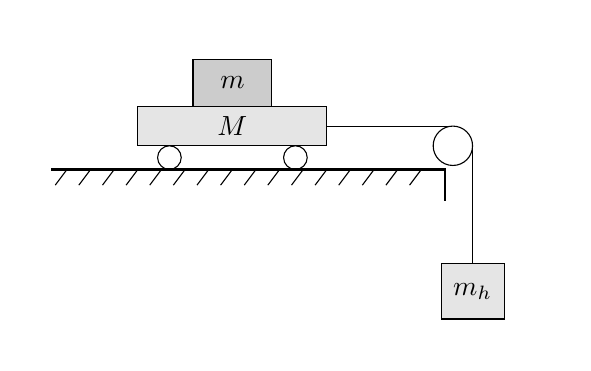
\begin{tikzpicture}
            \useasboundingbox (-0.8, -2.2) rectangle (6, 1.8);
            \draw[thick] (-0.5,0) -- (4.5,0) -- (4.5,-0.4);
            \foreach \x in {-0.3,0,...,4.4} \draw (\x,0) -- ++(-0.15,-0.2);
            \draw[fill=gray!20] (0.6,0.3) rectangle (3.0,0.8) node[midway] {$M$};
            \draw (1.0,0.15) circle (0.15);
            \draw (2.6,0.15) circle (0.15);
            \draw[fill=gray!40] (1.3,0.8) rectangle (2.3,1.4) node[midway] {$m$};
            \draw (3.0,0.55) -- (4.6,0.55);
            \draw[fill=white] (4.6,0.3) circle (0.25);
            \draw (4.85,0.3) -- (4.85,-1.2);
            \draw[fill=gray!20] (4.45,-1.9) rectangle (5.25,-1.2) node[midway] {$m_{h}$};
        \end{tikzpicture}
    \end{center}

    \begin{question}
        Wat is de grootst mogelijke versnelling van de wagen waarbij het blok niet over de wagen schuift?

        \[ a_{\max} = \answer[tolerance=0.02,onlineshowanswerbutton]{2.94} \, \mathrm{m/s^2} \]

        \begin{hint}
            Welke is de enige horizontale kracht op het blok? Zolang het blok niet schuift, heeft het dezelfde versnelling als de wagen.
        \end{hint}

        \begin{solution}\nl
            \underline{Gegevens:}
            \begin{align*}
                & M = 4{,}0 \, \mathrm{kg} & & m = 1{,}0 \, \mathrm{kg} \\
                & \mu_{s} = 0{,}30 & & \mu_{d} = 0{,}20 \\
                & g = 9{,}81 \, \mathrm{m/s^2} & &
            \end{align*}

            \underline{Gevraagd:} $a_{\max}$ \\

            \underline{Oplossing:}\\
            De enige horizontale kracht op het blok is de statische wrijving $F_{w,s}$ van de wagen. Die is hoogstens $\mu_{s} \cdot F_{N} = \mu_{s} \cdot m \cdot g$. Zonder schuiven heeft het blok dezelfde versnelling als de wagen:
            \begin{align*}
                F_{w,s} &= m \cdot a \leq \mu_{s} \cdot m \cdot g \\
                a_{\max} &= \mu_{s} \cdot g = 0{,}30 \cdot 9{,}81 \, \mathrm{m/s^2} = 2{,}943 \, \mathrm{m/s^2} \simeq 2{,}94 \, \mathrm{m/s^2}
            \end{align*}
        \end{solution}
    \end{question}

    \begin{question}
        Bereken de grootste massa $m_{h}$ waarbij het blok net niet over de wagen schuift.

        \[ m_{h,\max} = \answer[tolerance=0.03,onlineshowanswerbutton]{2.14} \, \mathrm{kg} \]

        \begin{hint}
            Op het grensgeval heeft het hele systeem de versnelling uit de vorige deelvraag. Bekijk de wagen met het blok erop als één geheel en het hangende blok afzonderlijk.
        \end{hint}

        \begin{solution}\nl
            \underline{Gevraagd:} $m_{h,\max}$ \\

            \underline{Oplossing:}\\
            Op het grensgeval versnellen wagen, blok en hangend blok met $a_{\max} = 2{,}943 \, \mathrm{m/s^2}$. Wagen en blok samen (positief naar rechts) en het hangende blok (positief omlaag):
            \begin{align*}
                F_{t} &= (M+m) \cdot a_{\max} \\
                m_{h} \cdot g - F_{t} &= m_{h} \cdot a_{\max}
            \end{align*}
            Combineren geeft:
            \begin{align*}
                m_{h} \cdot (g - a_{\max}) &= (M+m) \cdot a_{\max} \\
                m_{h} &= \frac{5{,}0 \, \mathrm{kg} \cdot 2{,}943 \, \mathrm{m/s^2}}{9{,}81 \, \mathrm{m/s^2} - 2{,}943 \, \mathrm{m/s^2}} = 2{,}143 \, \mathrm{kg} \simeq 2{,}14 \, \mathrm{kg}
            \end{align*}
        \end{solution}
    \end{question}

    \begin{question}
        Nu is $m_{h} = 3{,}0 \, \mathrm{kg}$. Bereken de grootte van de versnelling van het blok, van de wagen en de spankracht in het touw.

        \[ a_{\text{blok}} = \answer[tolerance=0.03,onlineshowanswerbutton]{1.96} \, \mathrm{m/s^2} \qquad a_{\text{wagen}} = \answer[tolerance=0.03,onlineshowanswerbutton]{3.92} \, \mathrm{m/s^2} \qquad F_{t} = \answer[tolerance=0.03,onlineshowanswerbutton]{17.7} \, \mathrm{N} \]

        \begin{hint}
            Controleer eerst of het blok nog met de wagen meebeweegt. Als het schuift, heeft het blok een andere versnelling dan de wagen. Welke zin heeft de wrijving op het blok en welke zin heeft de wrijving op de wagen? Wat zegt de derde wet?
        \end{hint}

        \begin{solution}\nl
            \underline{Gevraagd:} $a_{\text{blok}}$, $a_{\text{wagen}}$ en $F_{t}$ \\

            \underline{Oplossing:}\\
            Omdat $m_{h} = 3{,}0 \, \mathrm{kg} > 2{,}14 \, \mathrm{kg}$ schuift het blok over de wagen. De wrijving is dan dynamisch: $F_{w,d} = \mu_{d} \cdot m \cdot g = 0{,}20 \cdot 1{,}0 \, \mathrm{kg} \cdot 9{,}81 \, \mathrm{m/s^2} = 1{,}962 \, \mathrm{N}$. De wagen versnelt sterker dan het blok, dus het blok schuift naar achteren ten opzichte van de wagen. De wrijving op het blok wijst dus naar rechts en de wrijving op de wagen (derde wet) naar links.

            \begin{center}
            \begin{tikzpicture}
            \blokje[above left]{0}{0}{$m$}
            \kr[kracht]{0}{0}{0}{1.0}{right}{$\vec{\mathbf{F}}_{N}$}
            \kr[kracht]{0}{0}{0}{-1.0}{right}{$\vec{\mathbf{F}}_{z}$}
            \kr[kracht]{0}{0}{1.0}{0}{above}{$\vec{\mathbf{F}}_{w,d}$}
            \kr[versnelling]{0.3}{1.5}{0.8}{0}{above}{$\vec{\mathbf{a}}$}
            \blokje[above left]{6}{0}{$M$}
            \kr[kracht]{6}{0}{0}{1.47}{right}{$\vec{\mathbf{F}}_{N,\text{tafel}}$}
            \kr[kracht]{6.25}{0}{0}{-1.18}{right}{$\vec{\mathbf{F}}_{z}$}
            \kr[kracht]{5.75}{0}{0}{-0.29}{below left}{$\vec{\mathbf{F}}_{N,\text{blok}}$}
            \kr[kracht]{6}{0.05}{1.1}{0}{above}{$\vec{\mathbf{F}}_{t}$}
            \kr[kracht]{6}{-0.05}{-0.5}{0}{above left}{$\vec{\mathbf{F}}_{w,d}'$}
            \kr[versnelling]{6.3}{2.1}{1.0}{0}{above}{$\vec{\mathbf{a}}$}
            \end{tikzpicture}
            \end{center}

            Blok (positief naar rechts), wagen (positief naar rechts) en hangend blok (positief omlaag):
            \begin{align*}
                F_{w,d} &= m \cdot a_{\text{blok}} \\
                F_{t} - F_{w,d} &= M \cdot a_{\text{wagen}} \\
                m_{h} \cdot g - F_{t} &= m_{h} \cdot a_{\text{wagen}}
            \end{align*}
            Uit de eerste vergelijking:
            \[
                a_{\text{blok}} = \frac{1{,}962 \, \mathrm{N}}{1{,}0 \, \mathrm{kg}} = 1{,}962 \, \mathrm{m/s^2} \simeq 1{,}96 \, \mathrm{m/s^2}
            \]
            Optellen van de tweede en de derde vergelijking laat $F_{t}$ wegvallen:
            \begin{align*}
                a_{\text{wagen}} &= \frac{m_{h} \cdot g - F_{w,d}}{M + m_{h}} = \frac{3{,}0 \, \mathrm{kg} \cdot 9{,}81 \, \mathrm{m/s^2} - 1{,}962 \, \mathrm{N}}{4{,}0 \, \mathrm{kg} + 3{,}0 \, \mathrm{kg}} = 3{,}924 \, \mathrm{m/s^2} \simeq 3{,}92 \, \mathrm{m/s^2} \\
                F_{t} &= m_{h} \cdot (g - a_{\text{wagen}}) = 3{,}0 \, \mathrm{kg} \cdot (9{,}81 \, \mathrm{m/s^2} - 3{,}924 \, \mathrm{m/s^2}) = 17{,}658 \, \mathrm{N} \simeq 17{,}7 \, \mathrm{N}
            \end{align*}
            Controle: $a_{\text{wagen}} > a_{\text{blok}}$, dus de veronderstelling dat het blok achteruit schuift klopt.
        \end{solution}
    \end{question}
\end{exercise}
%———————————————————————————————————————

%———————————————————————————————————————
% OEFENING 6 (EXTRA): BEWEEGLIJKE KATROL
\begin{exercise}
    \textbf{Extra (verdieping).} Een blok met massa $m_{1}= 3{,}0 \, \mathrm{kg}$ ligt op een wrijvingsloze tafel. Aan het blok is een touw bevestigd dat over een vaste katrol aan de rand van de tafel loopt, vervolgens onder een beweeglijke katrol door gaat en met het andere uiteinde aan het plafond is vastgemaakt. Aan de beweeglijke katrol hangt een blok met massa $m_{2}= 4{,}0 \, \mathrm{kg}$. De massa van beide katrollen en van het touw is verwaarloosbaar. Het systeem wordt losgelaten.

    \begin{center}
        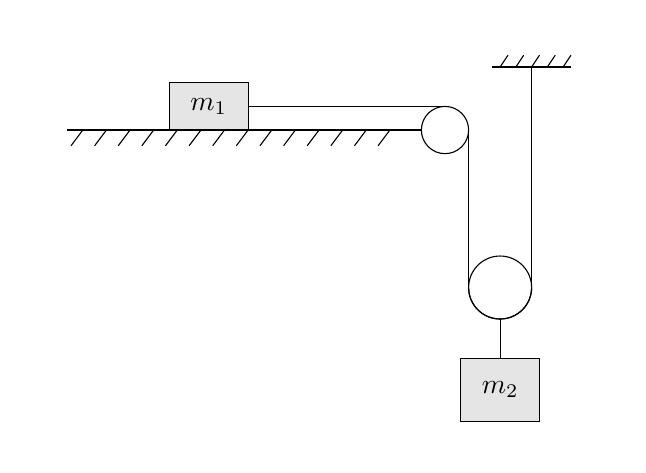
\begin{tikzpicture}
            \useasboundingbox (-1, -4) rectangle (6.5, 1.3);
            \draw[thick] (-0.5,0) -- (4.0,0);
            \foreach \x in {-0.3,0,...,3.9} \draw (\x,0) -- ++(-0.15,-0.2);
            \draw[fill=gray!20] (0.8,0) rectangle (1.8,0.6) node[midway] {$m_{1}$};
            \draw (1.8,0.3) -- (4.3,0.3);
            \draw (4.0,0) -- (4.3,0);
            \draw[fill=white] (4.3,0) circle (0.3);
            \draw (4.6,0) -- (4.6,-2);
            \draw[fill=white] (5.0,-2) circle (0.4);
            \draw (4.6,-2) arc[start angle=180,end angle=360,radius=0.4];
            \draw (5.4,-2) -- (5.4,0.8);
            \draw (4.9,0.8) -- (5.9,0.8);
            \foreach \x in {5.0,5.2,...,5.8} \draw (\x,0.8) -- ++(0.1,0.15);
            \draw (5.0,-2.4) -- (5.0,-2.9);
            \draw[fill=gray!20] (4.5,-3.7) rectangle (5.5,-2.9) node[midway] {$m_{2}$};
        \end{tikzpicture}
    \end{center}

    \begin{question}
        Wat is de verhouding tussen de grootte van de versnelling $a_{1}$ van blok 1 en de grootte van de versnelling $a_{2}$ van blok 2?

        \wordChoice{
            \choice{$a_{1} = a_{2}$}
            \choice[correct]{$a_{1} = 2 \cdot a_{2}$}
            \choice{$a_{1} = \frac{1}{2} \cdot a_{2}$}
        }

        \begin{hint}
            Stel dat blok 1 zich $1{,}0 \, \mathrm{m}$ naar rechts verplaatst. Hoeveel touw komt er dan beschikbaar voor de twee touwstukken die langs de beweeglijke katrol lopen? Wat betekent dat voor de zakbeweging van blok 2?
        \end{hint}

        \begin{solution}\nl
            De totale lengte van het touw is constant. Verplaatst blok 1 zich over een afstand $s$ naar de katrol toe, dan wordt het touwstuk op de tafel $s$ korter. Die lengte $s$ moet worden verdeeld over de twee verticale touwstukken aan de beweeglijke katrol. Elk wordt $\frac{s}{2}$ langer, dus de beweeglijke katrol en blok 2 zakken over $\frac{s}{2}$.

            Op elk tijdstip verplaatst blok 1 zich dus twee keer zoveel als blok 2, en dus ook $a_{1} = 2 \cdot a_{2}$.
        \end{solution}
    \end{question}

    \begin{question}
        Bereken de grootte van de versnelling van beide blokken.

        \[ a_{1} = \answer[tolerance=0.02,onlineshowanswerbutton]{4.9} \, \mathrm{m/s^2} \qquad a_{2} = \answer[tolerance=0.02,onlineshowanswerbutton]{2.45} \, \mathrm{m/s^2} \]

        \begin{hint}
            Het touw is overal even strak gespannen. Hoeveel touwstukken trekken er omhoog aan de beweeglijke katrol met blok 2? De katrol heeft geen massa, dus bekijk de katrol en blok 2 samen als één geheel.
        \end{hint}

        \begin{solution}\nl
            \underline{Gegevens:}
            \begin{align*}
                & m_{1} = 3{,}0 \, \mathrm{kg} & & m_{2} = 4{,}0 \, \mathrm{kg} \\
                & g = 9{,}81 \, \mathrm{m/s^2} & &
            \end{align*}

            \underline{Gevraagd:} $a_{1}$ en $a_{2}$ \\

            \underline{Oplossing:}\\
            \begin{center}
            \begin{tikzpicture}
            \blokje[left,xshift=-0.15cm]{0}{0}{$m_{1}$}
            \blokje[left,xshift=-0.15cm]{4.5}{0}{$m_{2}$}
            \kr[kracht]{0}{0.05}{0.74}{0}{above}{$\vec{\mathbf{F}}_{t}$}
            \kr[kracht]{0}{0}{0}{1.47}{right}{$\vec{\mathbf{F}}_{N}$}
            \kr[kracht]{0}{0}{0}{-1.47}{right}{$\vec{\mathbf{F}}_{z,1}$}
            \kr[kracht]{4.3}{0}{0}{0.74}{left}{$\vec{\mathbf{F}}_{t}$}
            \kr[kracht]{4.7}{0}{0}{0.74}{right}{$\vec{\mathbf{F}}_{t}$}
            \kr[kracht]{4.5}{0}{0}{-1.96}{right}{$\vec{\mathbf{F}}_{z,2}$}
            \kr[versnelling]{1.3}{0.8}{0.9}{0}{above}{$\vec{\mathbf{a}}$}
            \kr[versnelling]{5.4}{-0.4}{0}{-0.7}{right}{$\vec{\mathbf{a}}$}
            \end{tikzpicture}
            \end{center}

            In het hele touw is de spankracht $F_{t}$ overal gelijk. Op blok 1 werkt horizontaal enkel $F_{t}$ (positief naar rechts). Op de beweeglijke katrol met blok 2 werken twee touwstukken omhoog, elk met $F_{t}$, en de zwaartekracht omlaag (positief omlaag):
            \begin{align*}
                F_{t} &= m_{1} \cdot a_{1} \\
                m_{2} \cdot g - 2 \cdot F_{t} &= m_{2} \cdot a_{2}
            \end{align*}
            Met $a_{1} = 2 \cdot a_{2}$ wordt dit:
            \begin{align*}
                m_{2} \cdot g - 2 \cdot m_{1} \cdot 2 \cdot a_{2} &= m_{2} \cdot a_{2} \\
                a_{2} &= \frac{m_{2} \cdot g}{4 \cdot m_{1} + m_{2}} = \frac{4{,}0 \, \mathrm{kg} \cdot 9{,}81 \, \mathrm{m/s^2}}{4 \cdot 3{,}0 \, \mathrm{kg} + 4{,}0 \, \mathrm{kg}} = 2{,}4525 \, \mathrm{m/s^2} \simeq 2{,}45 \, \mathrm{m/s^2} \\
                a_{1} &= 2 \cdot a_{2} = 4{,}905 \, \mathrm{m/s^2} \simeq 4{,}9 \, \mathrm{m/s^2}
            \end{align*}
        \end{solution}
    \end{question}

    \begin{question}
        Bereken de spankracht in het touw.

        \[ F_{t} = \answer[tolerance=0.02,onlineshowanswerbutton]{14.7} \, \mathrm{N} \]

        \begin{hint}
            Is de spankracht even groot als de zwaartekracht op blok 2? Kies het blok waarvoor je de versnelling al kent en waarbij de spankracht de enige horizontale kracht is.
        \end{hint}

        \begin{solution}\nl
            \underline{Gevraagd:} $F_{t}$ \\

            \underline{Oplossing:}\\
            Uit de vergelijking van blok 1:
            \[
                F_{t} = m_{1} \cdot a_{1} = 3{,}0 \, \mathrm{kg} \cdot 4{,}905 \, \mathrm{m/s^2} = 14{,}715 \, \mathrm{N} \simeq 14{,}7 \, \mathrm{N}
            \]
            Controle: $2 \cdot F_{t} = 29{,}43 \, \mathrm{N}$ en $m_{2} \cdot g - 2 \cdot F_{t} = 39{,}24 \, \mathrm{N} - 29{,}43 \, \mathrm{N} = 9{,}81 \, \mathrm{N} = m_{2} \cdot a_{2}$. De spankracht is dus kleiner dan $m_{2} \cdot g = 39{,}24 \, \mathrm{N}$.
        \end{solution}
    \end{question}
\end{exercise}
%———————————————————————————————————————


%———————————————————————————————————————
% DEEL 2: DRADEN EN VEREN, VOOR EN NA HET DOORKNIPPEN OF LOSLATEN
%———————————————————————————————————————
\section{Draden en veren: voor en na het doorknippen of loslaten}

Een touw kan zijn lengte niet op een ogenblik veranderen en een veer ook niet. Daarom blijft de veerkracht net na het doorknippen of loslaten gelijk aan de veerkracht net ervoor, terwijl de spankracht in een touw wel meteen kan veranderen of verdwijnen.

%———————————————————————————————————————
% OEFENING 7: BLOK TUSSEN TWEE VEREN
\begin{exercise}
    Een blok met massa $m = 2{,}0 \, \mathrm{kg}$ hangt aan een bovenste veer met veerconstante $k_{1} = 3{,}0 \, \mathrm{N/cm}$ en is tegelijk met een onderste veer met veerconstante $k_{2} = 1{,}5 \, \mathrm{N/cm}$ vastgemaakt aan de vloer. Beide veren zijn uitgerekt. De bovenste veer is $12 \, \mathrm{cm}$ uitgerekt en het blok hangt in rust.

    \begin{center}
        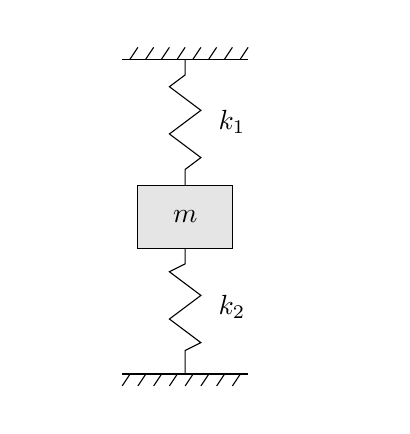
\begin{tikzpicture}
            \useasboundingbox (-2, -0.4) rectangle (2.5, 4.4);
            \draw[thick] (-0.8,0) -- (0.8,0);
            \foreach \x in {-0.7,-0.5,...,0.7} \draw (\x,0) -- ++(-0.1,-0.15);
            \draw (0,0) -- (0,0.3) -- (0.2,0.4) -- (-0.2,0.7) -- (0.2,1.0) -- (-0.2,1.3) -- (0,1.4) -- (0,1.6);
            \draw[fill=gray!20] (-0.6,1.6) rectangle (0.6,2.4) node[midway] {$m$};
            \draw (0,2.4) -- (0,2.6) -- (0.2,2.75) -- (-0.2,3.05) -- (0.2,3.35) -- (-0.2,3.65) -- (0,3.8) -- (0,4.0);
            \draw (-0.8,4.0) -- (0.8,4.0);
            \foreach \x in {-0.7,-0.5,...,0.7} \draw (\x,4.0) -- ++(0.1,0.15);
            \node[right] at (0.3,3.2) {$k_{1}$};
            \node[right] at (0.3,0.85) {$k_{2}$};
        \end{tikzpicture}
    \end{center}

    \begin{question}
        Bereken hoeveel de onderste veer is uitgerekt.

        \[ x_{2} = \answer[tolerance=0.03,onlineshowanswerbutton]{10.9} \, \mathrm{cm} \]

        \begin{hint}
            Teken alle krachten op het blok. De onderste veer is uitgerekt: in welke zin trekt ze aan het blok?
        \end{hint}

        \begin{solution}\nl
            \underline{Gegevens:}
            \begin{align*}
                & m = 2{,}0 \, \mathrm{kg} & & g = 9{,}81 \, \mathrm{m/s^2} \\
                & k_{1} = 3{,}0 \, \mathrm{N/cm} = 300 \, \mathrm{N/m} & & k_{2} = 1{,}5 \, \mathrm{N/cm} = 150 \, \mathrm{N/m} \\
                & x_{1} = 12 \, \mathrm{cm} = 0{,}12 \, \mathrm{m} & &
            \end{align*}

            \underline{Gevraagd:} $x_{2}$ \\

            \underline{Oplossing:}\\
            \begin{center}
            \begin{tikzpicture}[scale=1.5]
            \blokje[left,xshift=-0.15cm]{0}{0}{$m$}
            \kr[kracht]{0}{0}{0}{1.08}{right}{$\vec{\mathbf{F}}_{v,1}$}
            \kr[kracht]{-0.2}{0}{0}{-0.59}{left}{$\vec{\mathbf{F}}_{z}$}
            \kr[kracht]{0.2}{0}{0}{-0.49}{right}{$\vec{\mathbf{F}}_{v,2}$}
            \end{tikzpicture}
            \end{center}

            Beide veren zijn uitgerekt. De bovenste veer trekt het blok omhoog, de onderste veer trekt het blok omlaag. Samen met de zwaartekracht (omlaag) is het blok in evenwicht (positief omhoog):
            \begin{align*}
                F_{v,1} - m \cdot g - F_{v,2} &= 0 \\
                F_{v,1} &= k_{1} \cdot x_{1} = 300 \, \mathrm{N/m} \cdot 0{,}12 \, \mathrm{m} = 36 \, \mathrm{N} \\
                F_{v,2} &= 36 \, \mathrm{N} - 2{,}0 \, \mathrm{kg} \cdot 9{,}81 \, \mathrm{m/s^2} = 16{,}38 \, \mathrm{N} \\
                x_{2} &= \frac{F_{v,2}}{k_{2}} = \frac{16{,}38 \, \mathrm{N}}{150 \, \mathrm{N/m}} = 0{,}1092 \, \mathrm{m} \simeq 10{,}9 \, \mathrm{cm}
            \end{align*}
        \end{solution}
    \end{question}

    \begin{question}
        Het blok wordt plots losgemaakt van de onderste veer. Bereken de grootte van de versnelling van het blok net daarna.

        \[ a = \answer[tolerance=0.02,onlineshowanswerbutton]{8.19} \, \mathrm{m/s^2} \]

        \begin{hint}
            De bovenste veer is nog even lang als net voordien. Welke krachten werken er nu nog op het blok?
        \end{hint}

        \begin{solution}\nl
            \underline{Gevraagd:} $a$ \\

            \underline{Oplossing:}\\
            Net na het loskomen is $F_{v,1} = 36 \, \mathrm{N}$ nog ongewijzigd. De nettokracht (positief omhoog) is:
            \begin{align*}
                F_{v,1} - m \cdot g &= m \cdot a \\
                a &= \frac{36 \, \mathrm{N} - 2{,}0 \, \mathrm{kg} \cdot 9{,}81 \, \mathrm{m/s^2}}{2{,}0 \, \mathrm{kg}} = 8{,}19 \, \mathrm{m/s^2} \text{ (omhoog)}
            \end{align*}
        \end{solution}
    \end{question}

    \begin{question}
        Terug in de beginsituatie breekt in plaats daarvan de bovenste veer. Bereken de grootte van de versnelling van het blok net daarna.

        \[ a' = \answer[tolerance=0.02,onlineshowanswerbutton]{18.0} \, \mathrm{m/s^2} \]

        \begin{hint}
            Welke twee krachten wijzen nu allebei omlaag? Gebruik de gegevens uit de eerste deelvraag.
        \end{hint}

        \begin{solution}\nl
            \underline{Gevraagd:} $a'$ \\

            \underline{Oplossing:}\\
            De onderste veer trekt het blok nog steeds omlaag met $F_{v,2} = 16{,}38 \, \mathrm{N}$ en ook de zwaartekracht wijst omlaag (positief omlaag):
            \begin{align*}
                m \cdot g + F_{v,2} &= m \cdot a' \\
                a' &= \frac{2{,}0 \, \mathrm{kg} \cdot 9{,}81 \, \mathrm{m/s^2} + 16{,}38 \, \mathrm{N}}{2{,}0 \, \mathrm{kg}} = 18{,}0 \, \mathrm{m/s^2} \text{ (omlaag)}
            \end{align*}
        \end{solution}
    \end{question}
\end{exercise}
%———————————————————————————————————————

%———————————————————————————————————————
% OEFENING 8: ZWAAR TOUW VAN DRIE BLOKKEN
\begin{exercise}
    Drie blokken met massa $m_{1}= 2{,}0 \, \mathrm{kg}$, $m_{2}= 1{,}5 \, \mathrm{kg}$ en $m_{3}= 500 \, \mathrm{g}$ hangen onder elkaar aan touwen. Boven blok 1 hangt touw 1, tussen blok 1 en 2 hangt touw 2 en tussen blok 2 en 3 hangt touw 3. Iemand houdt touw 1 vast en trekt eraan met een kracht $\vec{\mathbf{F}}$.

    \begin{center}
        \begin{tikzpicture}
            \useasboundingbox (-2.5, -1, 0) rectangle (3, 4.2);
            \draw (0,2.6) -- (0,3.4);
            \draw[kracht] (0,3.4) -- (0,4.0) node[right] {$\vec{\mathbf{F}}$};
            \draw[fill=gray!20] (-0.6,1.8) rectangle (0.6,2.6) node[midway] {$m_{1}$};
            \draw (0,1.8) -- (0,1.2);
            \draw[fill=gray!20] (-0.5,0.4) rectangle (0.5,1.2) node[midway] {$m_{2}$};
            \draw (0,0.4) -- (0,-0.1);
            \draw[fill=gray!20] (-0.4,-0.7) rectangle (0.4,-0.1) node[midway] {$m_{3}$};
            \node[left] at (0,3.0) {touw 1};
            \node[left] at (0,1.5) {touw 2};
            \node[left] at (0,0.15) {touw 3};
        \end{tikzpicture}
    \end{center}

    \begin{question}
        Eerst houdt de persoon de blokken in rust. Bereken de spankracht in elk van de drie touwen.

        \[ F_{t,1} = \answer[tolerance=0.02,onlineshowanswerbutton]{39.2} \, \mathrm{N} \qquad F_{t,2} = \answer[tolerance=0.02,onlineshowanswerbutton]{19.6} \, \mathrm{N} \qquad F_{t,3} = \answer[tolerance=0.02,onlineshowanswerbutton]{4.9} \, \mathrm{N} \]

        \begin{hint}
            Elk touw draagt alles wat eronder hangt. Welke blokken hangen er onder touw 2?
        \end{hint}

        \begin{solution}\nl
            \underline{Gegevens:}
            \begin{align*}
                & m_{1} = 2{,}0 \, \mathrm{kg} & & m_{2} = 1{,}5 \, \mathrm{kg} \\
                & m_{3} = 500 \, \mathrm{g} = 0{,}50 \, \mathrm{kg} & & g = 9{,}81 \, \mathrm{m/s^2}
            \end{align*}

            \underline{Gevraagd:} $F_{t,1}$, $F_{t,2}$ en $F_{t,3}$ \\

            \underline{Oplossing:}\\
            Alles is in rust. Touw 3 draagt enkel blok 3, touw 2 draagt blok 2 en 3 en touw 1 draagt alle drie de blokken:
            \begin{align*}
                F_{t,3} &= m_{3} \cdot g = 0{,}50 \, \mathrm{kg} \cdot 9{,}81 \, \mathrm{m/s^2} = 4{,}905 \, \mathrm{N} \simeq 4{,}9 \, \mathrm{N} \\
                F_{t,2} &= (m_{2}+m_{3}) \cdot g = 2{,}0 \, \mathrm{kg} \cdot 9{,}81 \, \mathrm{m/s^2} = 19{,}62 \, \mathrm{N} \simeq 19{,}6 \, \mathrm{N} \\
                F_{t,1} &= (m_{1}+m_{2}+m_{3}) \cdot g = 4{,}0 \, \mathrm{kg} \cdot 9{,}81 \, \mathrm{m/s^2} = 39{,}24 \, \mathrm{N} \simeq 39{,}2 \, \mathrm{N}
            \end{align*}
        \end{solution}
    \end{question}

    \begin{question}
        Nu trekt de persoon de blokken met een constante versnelling van $2{,}0 \, \mathrm{m/s^2}$ omhoog. Bereken de spankracht in elk van de drie touwen.

        \[ F_{t,1} = \answer[tolerance=0.02,onlineshowanswerbutton]{47.2} \, \mathrm{N} \qquad F_{t,2} = \answer[tolerance=0.02,onlineshowanswerbutton]{23.6} \, \mathrm{N} \qquad F_{t,3} = \answer[tolerance=0.02,onlineshowanswerbutton]{5.9} \, \mathrm{N} \]

        \begin{hint}
            Alle blokken hebben dezelfde versnelling. Bekijk telkens het deelsysteem dat onder het touw hangt, net zoals in de eerste deelvraag.
        \end{hint}

        \begin{solution}\nl
            \underline{Gevraagd:} $F_{t,1}$, $F_{t,2}$ en $F_{t,3}$ bij $a = 2{,}0 \, \mathrm{m/s^2}$ omhoog \\

            \underline{Oplossing:}\\
            \begin{center}
            \begin{tikzpicture}[scale=1.5]
            \blokje[left,xshift=-0.15cm]{0}{0}{$m_{1}$}
            \blokje[left,xshift=-0.15cm]{3}{0}{$m_{2}$}
            \blokje[left,xshift=-0.15cm]{6}{0}{$m_{3}$}
            \kr[kracht]{0}{0}{0}{1.42}{right}{$\vec{\mathbf{F}}_{t,1}$}
            \kr[kracht]{-0.2}{0}{0}{-0.59}{left}{$\vec{\mathbf{F}}_{z,1}$}
            \kr[kracht]{0.2}{0}{0}{-0.71}{right}{$\vec{\mathbf{F}}_{t,2}$}
            \kr[kracht]{3}{0}{0}{0.71}{left}{$\vec{\mathbf{F}}_{t,2}$}
            \kr[kracht]{2.8}{0}{0}{-0.44}{left}{$\vec{\mathbf{F}}_{z,2}$}
            \kr[kracht]{3.2}{0}{0}{-0.18}{right}{$\vec{\mathbf{F}}_{t,3}$}
            \kr[kracht]{6}{0}{0}{0.18}{right}{$\vec{\mathbf{F}}_{t,3}$}
            \kr[kracht]{6}{0}{0}{-0.15}{right}{$\vec{\mathbf{F}}_{z,3}$}
            \kr[versnelling]{0.9}{0.2}{0}{0.8}{right}{$\vec{\mathbf{a}}$}
            \kr[versnelling]{3.9}{0.2}{0}{0.8}{right}{$\vec{\mathbf{a}}$}
            \kr[versnelling]{6.9}{0.2}{0}{0.8}{right}{$\vec{\mathbf{a}}$}
            \end{tikzpicture}
            \end{center}

            Voor elk deelsysteem onder een touw is de nettokracht (positief omhoog) gelijk aan de massa maal de versnelling:
            \begin{align*}
                F_{t,3} - m_{3} \cdot g &= m_{3} \cdot a \Rightarrow F_{t,3} = 0{,}50 \, \mathrm{kg} \cdot 11{,}81 \, \mathrm{m/s^2} = 5{,}905 \, \mathrm{N} \simeq 5{,}9 \, \mathrm{N} \\
                F_{t,2} - (m_{2}+m_{3}) \cdot g &= (m_{2}+m_{3}) \cdot a \Rightarrow F_{t,2} = 2{,}0 \, \mathrm{kg} \cdot 11{,}81 \, \mathrm{m/s^2} = 23{,}62 \, \mathrm{N} \simeq 23{,}6 \, \mathrm{N} \\
                F_{t,1} - (m_{1}+m_{2}+m_{3}) \cdot g &= (m_{1}+m_{2}+m_{3}) \cdot a \Rightarrow F_{t,1} = 4{,}0 \, \mathrm{kg} \cdot 11{,}81 \, \mathrm{m/s^2} = 47{,}24 \, \mathrm{N} \simeq 47{,}2 \, \mathrm{N}
            \end{align*}
            Hoe hoger het touw, hoe meer massa het moet versnellen, dus hoe groter de spankracht.
        \end{solution}
    \end{question}

    \begin{question}
        Terwijl de blokken met $2{,}0 \, \mathrm{m/s^2}$ omhoog versnellen, breekt touw 2. De persoon blijft met dezelfde kracht $F$ trekken. Bereken de grootte van de versnelling van blok 1 en van de blokken 2 en 3 net na het breken.

        \[ a_{1} = \answer[tolerance=0.02,onlineshowanswerbutton]{13.8} \, \mathrm{m/s^2} \qquad a_{2,3} = \answer[tolerance=0.02,onlineshowanswerbutton]{9.81} \, \mathrm{m/s^2} \]

        \begin{hint}
            Welke grootte had $F$ voor het breken? Welke krachten werken er na het breken nog op blok 1, en welke op blok 2 en 3?
        \end{hint}

        \begin{solution}\nl
            \underline{Gevraagd:} $a_{1}$ en $a_{2,3}$ \\

            \underline{Oplossing:}\\
            De kracht van de persoon is $F = F_{t,1} = 47{,}24 \, \mathrm{N}$ en blijft constant. Op blok 1 werken nu enkel $F$ (omhoog) en de zwaartekracht (omlaag):
            \begin{align*}
                F - m_{1} \cdot g &= m_{1} \cdot a_{1} \\
                a_{1} &= \frac{47{,}24 \, \mathrm{N} - 2{,}0 \, \mathrm{kg} \cdot 9{,}81 \, \mathrm{m/s^2}}{2{,}0 \, \mathrm{kg}} = 13{,}81 \, \mathrm{m/s^2} \simeq 13{,}8 \, \mathrm{m/s^2} \text{ (omhoog)}
            \end{align*}
            Blok 2 en 3 hangen nog aan elkaar via touw 3, maar er werkt geen andere kracht op dan de zwaartekracht. Beide blokken vallen vrij met $a_{2,3} = g = 9{,}81 \, \mathrm{m/s^2}$ (omlaag), en dus is $F_{t,3} = 0$.
        \end{solution}
    \end{question}
\end{exercise}
%———————————————————————————————————————

%———————————————————————————————————————
% OEFENING 9: VEER EN TOUW, DOORKNIPPEN
\begin{exercise}
    Een blok met massa $m_{1} = 1{,}5 \, \mathrm{kg}$ hangt aan een veer met veerconstante $k = 0{,}50 \, \mathrm{N/cm}$. Onder blok 1 hangt via een touw een blok met massa $m_{2} = 500 \, \mathrm{g}$. De massa van veer en touw is verwaarloosbaar.

    \begin{center}
        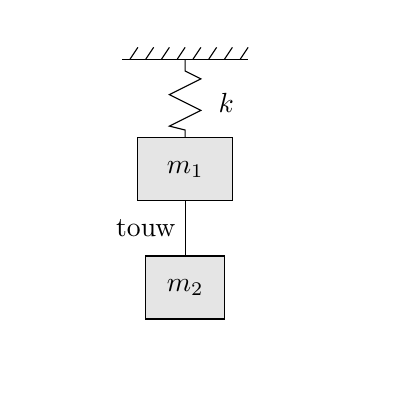
\begin{tikzpicture}
            \useasboundingbox (-2, -0.2) rectangle (2.5, 4.4);
            \draw (-0.8,4.0) -- (0.8,4.0);
            \foreach \x in {-0.7,-0.5,...,0.7} \draw (\x,4.0) -- ++(0.1,0.15);
            \draw (0,4.0) -- (0,3.85) -- (0.2,3.75) -- (-0.2,3.55) -- (0.2,3.35) -- (-0.2,3.15) -- (0,3.1) -- (0,3.0);
            \draw[fill=gray!20] (-0.6,2.2) rectangle (0.6,3.0) node[midway] {$m_{1}$};
            \draw (0,2.2) -- (0,1.5);
            \draw[fill=gray!20] (-0.5,0.7) rectangle (0.5,1.5) node[midway] {$m_{2}$};
            \node[right] at (0.3,3.45) {$k$};
            \node[left] at (0,1.85) {touw};
        \end{tikzpicture}
    \end{center}

    \begin{question}
        In rust: bereken de uitrekking van de veer en de spankracht in het touw.

        \[ x = \answer[tolerance=0.02,onlineshowanswerbutton]{39.2} \, \mathrm{cm} \qquad F_{t} = \answer[tolerance=0.02,onlineshowanswerbutton]{4.9} \, \mathrm{N} \]

        \begin{hint}
            Welk deelsysteem hangt er onder de veer en welk onder het touw?
        \end{hint}

        \begin{solution}\nl
            \underline{Gegevens:}
            \begin{align*}
                & m_{1} = 1{,}5 \, \mathrm{kg} & & m_{2} = 500 \, \mathrm{g} = 0{,}50 \, \mathrm{kg} \\
                & k = 0{,}50 \, \mathrm{N/cm} = 50 \, \mathrm{N/m} & & g = 9{,}81 \, \mathrm{m/s^2}
            \end{align*}

            \underline{Gevraagd:} $x$ en $F_{t}$ \\

            \underline{Oplossing:}\\
            De veer draagt beide blokken, het touw enkel blok 2:
            \begin{align*}
                k \cdot x &= (m_{1}+m_{2}) \cdot g \\
                x &= \frac{2{,}0 \, \mathrm{kg} \cdot 9{,}81 \, \mathrm{m/s^2}}{50 \, \mathrm{N/m}} = 0{,}3924 \, \mathrm{m} \simeq 39{,}2 \, \mathrm{cm} \\
                F_{t} &= m_{2} \cdot g = 0{,}50 \, \mathrm{kg} \cdot 9{,}81 \, \mathrm{m/s^2} = 4{,}905 \, \mathrm{N} \simeq 4{,}9 \, \mathrm{N}
            \end{align*}
        \end{solution}
    \end{question}

    \begin{question}
        Het touw wordt doorgeknipt. Bereken de grootte van de versnelling van blok 1 en van blok 2 net daarna.

        \[ a_{1} = \answer[tolerance=0.02,onlineshowanswerbutton]{3.27} \, \mathrm{m/s^2} \qquad a_{2} = \answer[tolerance=0.02,onlineshowanswerbutton]{9.81} \, \mathrm{m/s^2} \]

        \begin{hint}
            Welke krachten werken er op blok 1 vlak na het doorknippen? Is de veerkracht al veranderd?
        \end{hint}

        \begin{solution}\nl
            \underline{Gevraagd:} $a_{1}$ en $a_{2}$ \\

            \underline{Oplossing:}\\
            \begin{center}
            \begin{tikzpicture}[scale=1.5]
            \blokje[left,xshift=-0.15cm]{0}{0}{$m_{1}$}
            \blokje[left,xshift=-0.15cm]{3}{0}{$m_{2}$}
            \kr[kracht]{0}{0}{0}{0.59}{right}{$\vec{\mathbf{F}}_{v}$}
            \kr[kracht]{0}{0}{0}{-0.44}{right}{$\vec{\mathbf{F}}_{z,1}$}
            \kr[kracht]{3}{0}{0}{-0.15}{right}{$\vec{\mathbf{F}}_{z,2}$}
            \kr[versnelling]{0.9}{0.2}{0}{0.8}{right}{$\vec{\mathbf{a}}$}
            \kr[versnelling]{3.9}{-0.2}{0}{-0.8}{right}{$\vec{\mathbf{a}}$}
            \end{tikzpicture}
            \end{center}

            Net na het doorknippen is de veerkracht nog $F_{v} = (m_{1}+m_{2}) \cdot g = 19{,}62 \, \mathrm{N}$ (omhoog). Blok 2 valt vrij: $a_{2} = g = 9{,}81 \, \mathrm{m/s^2}$ (omlaag). Voor blok 1 (positief omhoog):
            \begin{align*}
                F_{v} - m_{1} \cdot g &= m_{1} \cdot a_{1} \\
                a_{1} &= \frac{19{,}62 \, \mathrm{N} - 1{,}5 \, \mathrm{kg} \cdot 9{,}81 \, \mathrm{m/s^2}}{1{,}5 \, \mathrm{kg}} = 3{,}27 \, \mathrm{m/s^2} \text{ (omhoog)}
            \end{align*}
        \end{solution}
    \end{question}

    \begin{question}
        Blok 1 beweegt na het doorknippen omhoog. Bereken de versnelling van blok 1 op het moment dat de veer nog slechts $25 \, \mathrm{cm}$ is uitgerekt, en geef de zin ervan.

        \[ a = \answer[tolerance=0.03,onlineshowanswerbutton]{1.48} \, \mathrm{m/s^2} \]

        Zin van de versnelling: \wordChoice{
            \choice[correct]{omlaag}
            \choice{omhoog}
        }

        \begin{hint}
            Bij welke uitrekking zou blok 1 alleen in evenwicht hangen? Vergelijk daarmee de nu kleinere uitrekking.
        \end{hint}

        \begin{solution}\nl
            \underline{Gevraagd:} $a$ bij $x = 25 \, \mathrm{cm}$ \\

            \underline{Oplossing:}\\
            Bij $x = 25 \, \mathrm{cm} = 0{,}25 \, \mathrm{m}$ is de veerkracht $F_{v} = 50 \, \mathrm{N/m} \cdot 0{,}25 \, \mathrm{m} = 12{,}5 \, \mathrm{N}$. Dat is kleiner dan de zwaartekracht $m_{1} \cdot g = 14{,}715 \, \mathrm{N}$ (het nieuwe evenwichtspunt ligt bij $\frac{m_{1} \cdot g}{k} = 29{,}4 \, \mathrm{cm}$). De nettokracht wijst dus omlaag (positief omlaag):
            \begin{align*}
                m_{1} \cdot g - F_{v} &= m_{1} \cdot a \\
                a &= \frac{14{,}715 \, \mathrm{N} - 12{,}5 \, \mathrm{N}}{1{,}5 \, \mathrm{kg}} = 1{,}477 \, \mathrm{m/s^2} \simeq 1{,}48 \, \mathrm{m/s^2} \text{ (omlaag)}
            \end{align*}
            Blok 1 versnelt eerst omhoog, gaat voorbij het evenwichtspunt en wordt dan afgeremd.
        \end{solution}
    \end{question}
\end{exercise}
%———————————————————————————————————————

%———————————————————————————————————————
% OEFENING 10: ATWOOD MET VEER, LOSLATEN
\begin{exercise}
    Over een vaste katrol loopt een touw. Aan de linkerkant hangt een blok met massa $m_{1} = 3{,}0 \, \mathrm{kg}$, dat rust op een steun. Aan de rechterkant hangt een blok met massa $m_{2} = 1{,}0 \, \mathrm{kg}$. Onder blok 2 hangt via een veer met veerconstante $k = 1{,}0 \, \mathrm{N/cm}$ een blok met massa $m_{3} = 800 \, \mathrm{g}$. Het systeem hangt in rust en het touw is gespannen.

    \begin{center}
        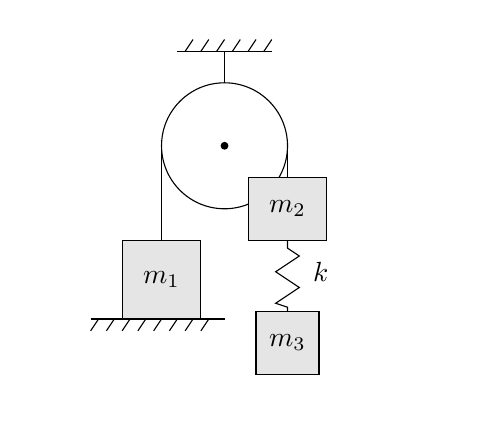
\begin{tikzpicture}
            \useasboundingbox (-2.5, -0.3) rectangle (3, 4.5);
            \draw (-0.6,4.2) -- (0.6,4.2);
            \foreach \x in {-0.5,-0.3,...,0.5} \draw (\x,4.2) -- ++(0.1,0.15);
            \draw (0,4.2) -- (0,3);
            \draw[fill=white] (0,3) circle (0.8);
            \fill (0,3) circle (0.05);
            \draw (-0.8,3) -- (-0.8,1.8);
            \draw (0.8,3) -- (0.8,2.6);
            \draw[fill=gray!20] (-1.3,0.8) rectangle (-0.3,1.8) node[midway] {$m_{1}$};
            \draw[thick] (-1.7,0.8) -- (0,0.8);
            \foreach \x in {-1.6,-1.4,...,-0.1} \draw (\x,0.8) -- ++(-0.1,-0.15);
            \draw[fill=gray!20] (0.3,1.8) rectangle (1.3,2.6) node[midway] {$m_{2}$};
            \draw (0.8,1.8) -- (0.8,1.7) -- (0.95,1.6) -- (0.65,1.4) -- (0.95,1.2) -- (0.65,1.0) -- (0.8,0.95) -- (0.8,0.9);
            \draw[fill=gray!20] (0.4,0.1) rectangle (1.2,0.9) node[midway] {$m_{3}$};
            \node[right] at (1.0,1.4) {$k$};
        \end{tikzpicture}
    \end{center}

    \begin{question}
        Bereken de uitrekking van de veer en de spankracht in het touw terwijl alles in rust is.

        \[ x = \answer[tolerance=0.02,onlineshowanswerbutton]{7.85} \, \mathrm{cm} \qquad F_{t} = \answer[tolerance=0.02,onlineshowanswerbutton]{17.7} \, \mathrm{N} \]

        \begin{hint}
            Welke blokken hangen er onder de veer, en welke onder het touw aan de rechterkant?
        \end{hint}

        \begin{solution}\nl
            \underline{Gegevens:}
            \begin{align*}
                & m_{1} = 3{,}0 \, \mathrm{kg} & & m_{2} = 1{,}0 \, \mathrm{kg} \\
                & m_{3} = 800 \, \mathrm{g} = 0{,}80 \, \mathrm{kg} & & k = 1{,}0 \, \mathrm{N/cm} = 100 \, \mathrm{N/m} \\
                & g = 9{,}81 \, \mathrm{m/s^2} & &
            \end{align*}

            \underline{Gevraagd:} $x$ en $F_{t}$ \\

            \underline{Oplossing:}\\
            Blok 3 is in rust: $F_{v} = m_{3} \cdot g = 7{,}848 \, \mathrm{N}$ en dus
            \[
                x = \frac{F_{v}}{k} = \frac{7{,}848 \, \mathrm{N}}{100 \, \mathrm{N/m}} = 0{,}07848 \, \mathrm{m} \simeq 7{,}85 \, \mathrm{cm}
            \]
            De rechterkant (blok 2, veer en blok 3) is in rust en het touw draagt blok 2 en 3:
            \[
                F_{t} = (m_{2}+m_{3}) \cdot g = 1{,}8 \, \mathrm{kg} \cdot 9{,}81 \, \mathrm{m/s^2} = 17{,}658 \, \mathrm{N} \simeq 17{,}7 \, \mathrm{N}
            \]
        \end{solution}
    \end{question}

    \begin{question}
        Bereken de grootte van de kracht die de steun uitoefent op blok 1.

        \[ F_{N} = \answer[tolerance=0.02,onlineshowanswerbutton]{11.8} \, \mathrm{N} \]

        \begin{hint}
            Blok 1 is in rust. Welke krachten werken er op blok 1 in verticale zin?
        \end{hint}

        \begin{solution}\nl
            \underline{Gevraagd:} $F_{N}$ \\

            \underline{Oplossing:}\\
            Op blok 1 werken de spankracht en de normaalkracht omhoog en de zwaartekracht omlaag:
            \begin{align*}
                F_{N} + F_{t} - m_{1} \cdot g &= 0 \\
                F_{N} &= 3{,}0 \, \mathrm{kg} \cdot 9{,}81 \, \mathrm{m/s^2} - 17{,}658 \, \mathrm{N} = 11{,}772 \, \mathrm{N} \simeq 11{,}8 \, \mathrm{N}
            \end{align*}
        \end{solution}
    \end{question}

    \begin{question}
        De steun wordt plots weggehaald. Bereken net daarna de grootte van de versnelling van blok 1 en 2, de versnelling van blok 3 en de spankracht in het touw.

        \[ a_{1,2} = \answer[tolerance=0.02,onlineshowanswerbutton]{2.94} \, \mathrm{m/s^2} \qquad a_{3} = \answer[tolerance=0.02,onlineshowanswerbutton]{0} \, \mathrm{m/s^2} \qquad F_{t}' = \answer[tolerance=0.02,onlineshowanswerbutton]{20.6} \, \mathrm{N} \]

        \begin{hint}
            De veer heeft nog dezelfde lengte. Wat betekent dat voor de krachten op blok 3? Welke krachten werken er op blok 2 en welke op blok 1?
        \end{hint}

        \begin{solution}\nl
            \underline{Gevraagd:} $a_{1,2}$, $a_{3}$ en $F_{t}'$ \\

            \underline{Oplossing:}\\
            \begin{center}
            \begin{tikzpicture}[scale=1.5]
            \blokje[left,xshift=-0.15cm]{0}{0}{$m_{1}$}
            \blokje[left,xshift=-0.15cm]{3}{0}{$m_{2}$}
            \blokje[left,xshift=-0.15cm]{6}{0}{$m_{3}$}
            \kr[kracht]{0}{0}{0}{0.62}{right}{$\vec{\mathbf{F}}_{t}$}
            \kr[kracht]{0}{0}{0}{-0.88}{right}{$\vec{\mathbf{F}}_{z,1}$}
            \kr[kracht]{3}{0}{0}{0.62}{left}{$\vec{\mathbf{F}}_{t}$}
            \kr[kracht]{2.8}{0}{0}{-0.29}{left}{$\vec{\mathbf{F}}_{z,2}$}
            \kr[kracht]{3.2}{0}{0}{-0.24}{right}{$\vec{\mathbf{F}}_{v}$}
            \kr[kracht]{6}{0}{0}{0.24}{left}{$\vec{\mathbf{F}}_{v}$}
            \kr[kracht]{6.2}{0}{0}{-0.24}{right}{$\vec{\mathbf{F}}_{z,3}$}
            \kr[versnelling]{0.9}{-0.2}{0}{-0.8}{right}{$\vec{\mathbf{a}}$}
            \kr[versnelling]{3.9}{0.2}{0}{0.8}{right}{$\vec{\mathbf{a}}$}
            \end{tikzpicture}
            \end{center}

            Net na het wegnemen van de steun is de veerkracht nog $F_{v} = 7{,}848 \, \mathrm{N}$. Op blok 3 compenseren veerkracht en zwaartekracht elkaar, dus $a_{3} = 0$.

            Blok 1 zakt en blok 2 stijgt met dezelfde versnelling. Op blok 2 werken de spankracht (omhoog), de zwaartekracht en de veerkracht van de uitgerekte veer (beide omlaag):
            \begin{align*}
                m_{1} \cdot g - F_{t}' &= m_{1} \cdot a_{1,2} \\
                F_{t}' - m_{2} \cdot g - F_{v} &= m_{2} \cdot a_{1,2}
            \end{align*}
            Optellen laat $F_{t}'$ wegvallen:
            \begin{align*}
                a_{1,2} &= \frac{m_{1} \cdot g - m_{2} \cdot g - F_{v}}{m_{1}+m_{2}} = \frac{29{,}43 \, \mathrm{N} - 9{,}81 \, \mathrm{N} - 7{,}848 \, \mathrm{N}}{4{,}0 \, \mathrm{kg}} = 2{,}943 \, \mathrm{m/s^2} \simeq 2{,}94 \, \mathrm{m/s^2} \\
                F_{t}' &= m_{1} \cdot (g - a_{1,2}) = 3{,}0 \, \mathrm{kg} \cdot (9{,}81 \, \mathrm{m/s^2} - 2{,}943 \, \mathrm{m/s^2}) = 20{,}601 \, \mathrm{N} \simeq 20{,}6 \, \mathrm{N}
            \end{align*}
            De spankracht is groter geworden dan in rust ($17{,}7 \, \mathrm{N}$) omdat blok 2 nu omhoog versnelt.
        \end{solution}
    \end{question}
\end{exercise}
%———————————————————————————————————————

\end{document}